\documentclass[a4paper]{article}
\usepackage[
    lecture,
    course={Lineare Algebra~I},
    code={V1G3},
    lecturer={Prof.~Dr.\ Jan Schröer},
    term={WS~2021/2022}
]{tienuni}

\overfullrule3cm

\begin{document}
\maketitle
\tableofcontents

\section{Grundlagen}

\subsection{Mengen}

Wir wollen uns mit einer sehr naiven, aber für unsere Zwecke ausreichenden, Mengenbegriff beschäftigen. Was eine Menge wirklich ist, erfahren wir von den Logikern und Mengentheoretikern.

\begin{definition}[naive Menge]
    Eine Menge~$M$ ist eine Zusammenfassung von verschiedenen Objekten, welche dann Elemente genannt werden, zu einem Objekt.
\end{definition}

\begin{example}\leavevmode
    \begin{itemize}
        \item $\N \coloneqq \mset{0, 1, 2, \dots}$, die Menge der \emph{natürliche Zahlen}. In dieser Vorlesung gehört die Null dazu.
        \item $\Z \coloneqq \mset{\dots, -2, -1, 0, 1, 2, \dots}$, die Menge der \emph{ganze Zahlen}.
        \item $\Q \coloneqq \mset{a/b \mid a, b \in \Z, b \geq 1}$, die Menge der \emph{rationale Zahlen}.
        \item $\R$,~die Menge der \emph{rationalen Zahlen}.
        \item $\C$,~die Menge der \emph{komplexen Zahlen}.
        \item $\varnothing$,~die leere Menge, die per Definition keine Elemente enthält.
    \end{itemize}
\end{example}

\begin{notation}[Quantoren, Mengenschreibweise, Relationen]
    Einige häufig verwendete Symbole
    \begin{itemize}
        \item $(\dots) \coloneqq (\dots)$ definiert das, was links steht, durch das, was rechts steht.
        \item $\forall$~bedeutet "`für alle"'.
        \item $\exists$~bedeutet "`es existiert"'.
        \item Wenn~$M$ eine Menge ist, bezeichnet $\abs{M}$ die Anzahl der Elemente in~$M$ (\emph{Kardinalität}). Für die leere Menge ist $\abs{\varnothing} = 0$.
        \item Eine Menge~$M$ heißt \emph{$n$"~elementig}, falls~$\abs{M} = n$ ($n \geq 0$).
        \item Allgemein notieren wir Mengen bspw.\ durch
              \begin{equation*}
                  \mset{21, 35} = \mset{x \in \N \mid 5 \leq x \leq 40, 7 \mid x, x \in \mset{7, 14, 28}}.
              \end{equation*}

              \begin{itemize}
                  \item[$\mset{\;}$] sind Mengenklammern.
                  \item[$\mid$]steht oft für "`mit der Eigenschaft"'. In unserem Beispiel heißt das "`alle $x \in \N$ mit der Eigenschaft, dass \dots"'
                  \item[$,$] steht oft für "`und"', eine logische Verknüpfung der Bedingungen bzw.\ Eigenschaften.
                  \item[$\in$] steht für "`ist Element von"'. Hingegen ist~$\notin$~"`ist kein Element von"'.
                  \item[$=$] steht für "`gleich"', d.\,h.\ links und rechts steht das gleiche und können gegenseitig ausgetauscht werden. Analog ist $\neq$~"`ungleich"'.
              \end{itemize}
        \item $\leq$,~$<$, $\geq$,~$>$ sind "`kleiner gleich"', "`(echt) kleiner"', "`größer gleich"', "`(echt) größer"'.
    \end{itemize}
\end{notation}

\begin{remark}
    Die Reihenfolge und Vielfachheit der Elemente in der Aufzählung von Mengen ist egal. Deshalb ist $\mset{1, 2, 3} = \mset{2, 1, 3} = \mset{1, 1, 3, 2, 3}$.
\end{remark}

\begin{definition}[Teilmenge]
    Seien $A$~und~$B$ Mengen. Dann ist
    \begin{itemize}
        \item $A$~eine \emph{Teilmenge} von~$B$, falls $x \in B$ für alle~$x \in A$, geschrieben $A \subseteq B$, und
        \item $A$~eine \emph{echte Teilmenge} von~$B$, falls $A \subseteq B$, aber~$A \neq B$, geschrieben $A \subset B$.
    \end{itemize}
\end{definition}

\begin{remark}
    Für jede Menge~$M$ gilt $\varnothing \subseteq M$, aber $\varnothing \in M$ im Allgemeinen nicht.
\end{remark}

Weiterhin definieren wir

\begin{definition}[Mengenoperatoren]
    Für Mengen $A$~und~$B$ seien
    \begin{itemize}
        \item $A \cap B \coloneqq \mset{x \mid x \in A, x \in B}$ der \emph{Durchschnitt} von $A$~und~$B$,
        \item $A \cup B \coloneqq \mset{x \mid x \in A \text{ oder } x \in B}$ die \emph{Vereinigung} von $A$~und~$B$,
        \item $A \setminus B \coloneqq \mset{x \mid x \in A, x \notin B}$ die \emph{Mengendifferenz} von $A$~und~$B$,
        \item $\powerset(A) \coloneqq \mset{U \mid U \subseteq A}$ die \emph{Potenzmenge} von~$A$.
    \end{itemize}
\end{definition}

\begin{definition}[Indexmenge]
    Sei $I$~eine \emph{Indexmenge}, d.\,h.\ für jedes~$i \in I$ ist $A_i$~eine Menge. Dann sind
    \begin{equation*}
        \bigcap_{i \in I} A_i \coloneqq \mset{x \mid x \in A_i \text{ für alle } i \in I} \qquad\text{und}\qquad \bigcup_{i \in I} A_i \coloneqq \mset{x \mid \text{es gibt ein } i \in I \text{ mit } x \in A_i}
    \end{equation*}
    der \emph{Durchschnitt} bzw.\ \emph{Vereinigung} der Mengen~$A_i$ über die Indexmenge~$I$.
\end{definition}

\begin{example}\leavevmode
    \begin{itemize}
        \item $\powerset(\mset{1, 2}) = \mset{\varnothing, \mset{1}, \mset{2}, \mset{1, 2}}$ ist 4"~elementig.
        \item $\mset{1, 2, 3} \cup \mset{2, 3} = \mset{1, 2, 3}$.
        \item $\mset{1, 2} \setminus \mset{1, 3} = \mset{2}$. Die Differenzmenge~$A \setminus B$ nimmt $B$ von~$A$ weg.
        \item $\varnothing \cup \mset{1, 2} = \mset{1, 2} \neq \mset{\varnothing, 1, 2} = \mset{\varnothing} \cup \mset{1, 2}$. Die Vereinigung mit der leeren Menge macht nichts.
        \item $\mset{\varnothing, \mset{1, 2, 3, 4}}$ ist 2"~elementig, wohingegen $\mset{\varepsilon, 1, 2, 3, 4}$ 5"~elementig ist.
    \end{itemize}
\end{example}

\begin{definition}[Paar]
    Ein \emph{Paar} (oder \emph{2"~Tupel}) besteht aus der Angabe eines ersten Elements~$a$ und eines zweiten Elements~$b$. Wir schreiben~$(a, b)$.
\end{definition}

\begin{remark}
    Bei Paaren ist (im Gegensatz zu Mengen) die Reihenfolge wichtig. Es gilt $(a, b) = (b, a)$ genau dann, wenn~$a = b$: \emph{Achtung}: $(a, a) \neq \mset{a, a} = \mset{a}$.
\end{remark}

\begin{definition}[\textsc{kartesisches} Produkt, Tupel]
    Das \emph{\textsc{kartesische} Produkt} zweier Mengen $A$~und~$B$ ist $A \times B \coloneqq \mset{(a, b) \mid a \in A, b \in B}$.

    Für Mengen $A_1, A_2, \dots, A_n$ ist das \emph{\textsc{kartesische} Produkt}
    \begin{equation*}
        A_1 \times \dots \times A_n \coloneqq \mset{(a_1, \dots, a_n) \mid a_i \in A_i \text{ für } 1 \leq i \leq n},
    \end{equation*}
    dessen Elemente \emph{$n$"~Tupel} genannt werden.

    Sei~$A$ eine Menge und~$n \geq 1$. Dann ist
    \begin{equation*}
        A^n \coloneqq \underbrace{A \times \dots \times A}_{n \text{ mal}}
    \end{equation*}
    das \emph{$n$"~fache \textsc{kartesische} Produkt} von~$A$.
\end{definition}

\begin{remark}
    Zwei Tupel sind gleich, wenn sie gleich viele \emph{Einträge} bzw.\ \emph{Komponenten} haben und wenn an jeder Stelle die Komponenten gleich sind.
\end{remark}

\begin{notation}
    Die $n$"~Tupel $(a_1, a_2, \dots, a_n)$ schreiben wir oft auch senkrecht auf:
    \begin{equation*}
        \begin{pmatrix}
            a_1 \\ a_2 \\ \vdots \\ a_n
        \end{pmatrix}
    \end{equation*}
\end{notation}

\begin{example}
    Sind $A$,~$B$ und~$C$ Mengen, dann sind die Elemente in~$A \times B \times C$ 3"~Tupel der Form $(a, b, c)$, während die Elemente in~$(A \times B) \times C$ 2"~Tupel der Form $((a, b), c)$.
\end{example}

\subsection{Logik}

\begin{definition}[Implikation, Äquivalenz]
    Seien $A$,~$B$ und~$C$ Aussagen. Dann bedeuten
    \begin{itemize}
        \item $A \implies B$ "`$A$~impliziert~$B$"', "`aus~$A$ folgt~$B$"',
        \item $A \iff B$ "`$A$~genau dann, wenn~$B$"', "`$A$~und~$B$ sind äquivalent"', d.\,h.\ $A \implies B$ und $B \implies A$,
        \item $\neg A$, "`nicht~$A$"'.
    \end{itemize}
\end{definition}

Zwei Schlussregeln, die wir oft verwenden werden:

\begin{theorem}[Syllogismus, Kontraposition]\label{thm:deductionrules}\leavevmode
    \begin{itemize}
        \item Aus~$A \implies B$ und~$B \implies C$ folgt~$A \implies C$ (\emph{Syllogismus}).
        \item Es gilt~$A \implies B$ genau dann, wenn~$\neg B \implies \neg A$ (\emph{Kontraposition}).
    \end{itemize}
\end{theorem}

\begin{example}
    \begin{gather*}
        \underbrace{\text{"`Wenn es regnet,}}_{\displaystyle A}\; \underbrace{\text{ist die Straße nass."'}}_{\displaystyle B} \qquad (A \implies B) \\
        \shortintertext{ist äquivalent zu} \\
        \underbrace{\text{"`Wenn die Straße nicht nass ist,}}_{\displaystyle\neg B}\; \underbrace{\text{dann regnet es nicht."'}}_{\displaystyle\neg A} \qquad (\neg B \implies \neg A)
    \end{gather*}
\end{example}

\subsubsection{Beweis durch Induktion}

Für jedes natürliche~$n \geq 1$ sei $A(n)$~eine Aussage. Wenn das Ziel ist, $A(n)$ für alle~$n \geq 1$ zu zeigen, dann kann \emph{vollständige Induktion} helfen. Die Beweisstrategie:
\begin{itemize}
    \item \emph{Induktionsanfang}: Wir zeigen, dass $A(1)$~richtig ist.
    \item \emph{Induktionsschritt}: Wir nehmen an, dass $A(n)$~richtig ist. Damit beweisen wir, dass auch $A(n+1)$~richtig ist.
\end{itemize}

Das Beweisprinzip basiert auf dem Dominoeffekt: Mit dem Induktionsanfang ist~$A(1)$ wahr. Mit dem Induktionsschritt folgt aus~$A(1)$ auch~$A(2)$. Wieder mit dem Induktionsschritt folgt aus~$A(2)$ auch~$A(3)$ usw. Damit haben wir die Aussagen~$A(n)$ für alle~$n \geq 1$ gezeigt.

\begin{example}\leavevmode
    \begin{itemize}
        \item Für alle~$n \geq 1$ gilt $A(n)\colon \sum_{k=1}^n (2k-1) = n^2$.
              \begin{itemize}
                  \item \emph{Induktionsanfang} ($n = 1$): $2 \cdot 1 - 1 = 1^2$ ist wahr und deshalb auch~$A(1)$.
                  \item \emph{Induktionsschritt}: Es gilt
                        \begin{equation*}
                            \sum_{k=1}^{n+1} (2k-1) = \paren*{\sum_{k=1}^n (2k-1)} + (2(n+1) - 1) = n^2 + 2n + 1 = (n+1)^2.
                        \end{equation*}
                        Dabei verwendeten wir für die zweite Gleichheit die Induktionsvoraussetzung. Folglich gilt~$A(n+1)$.
              \end{itemize}
        \item Ein falscher Induktionsbeweis: Wir behaupten, dass $A(n)\colon (7 \text{ teilt } 10^n)$ für alle~$n \geq 1$ gilt.
              \begin{itemize}
                  \item \emph{Induktionsschritt}: Angenommen $A(n)$ ist wahr, d.\,h.\ es gilt $10^n = 7a$ für ein~$a \geq 1$ in~$\N$. Dann gilt auch $10^{n+1} = 10 \cdot 10^n = 10 \cdot 7a$. Also gilt~$A(n+1)$.
                  \item \emph{Induktionsanfang}: Aber~$A(1)$ ist falsch!
              \end{itemize}
    \end{itemize}
\end{example}

\subsubsection{Beweis durch Widerspruch}

Das Beweisprinzip ist, das Gegenteil der Behauptung anzunehmen und das auf einen Widerspruch mit der Voraussetzung zu führen. Folglich war die Annahme falsch und die Behauptung richtig.

\begin{example}
    \emph{Behauptung}: $\sqrt{2} \notin \Q$.

    \emph{Beweis}: Angenommen $\sqrt{2} \in \Q$, d.\,h.\ Es gibt $a, b \in \Z$, $b \geq 1$ mit~$\sqrt{2} = a/b$. Wir können annehmen, dass $a$~und~$b$ teilerfremd sind (also der Bruch vollständig gekürzt ist).

    Quadrieren liefert $2 = a^2/b^2 \iff 2b^2 = a^2$. Damit sind $a^2$~und~$a$ durch 2~teilbar, insbesondere auch~$a^2$ durch $2\cdot2 = 4$ teilbar. Somit teilt~4 auch~$2b^2$, also sind $b^2$~und~$b$ auch durch 2~teilbar (aufgrund der Eindeutigkeit der Primfaktorzerlegung). Das bedeutet, dass $a$~und~$b$ durch 2~teilbar sind, was im Widerpsruch zur Teilerfremdheit steht.
\end{example}

\subsubsection{Gleichheit von Mengen}

\begin{remark}
    Zwei Mengen sind \emph{gleich}, wenn sie dieselben Elemente besitzen.
\end{remark}

Seien $A$~und~$B$ zwei Mengen. Um zu beweisen, dass~$A=B$ ist, muss man zum Einen~$A \subseteq B$ und zum Anderen~$B \subseteq A$ zeigen. Der Beweis ist im Regelfall also zweiteilig!

\subsection{Abbildungen}

Die Idee hinter Abbildungen ist es, Mengen in Beziehung zu setzen.\footnote{Eigentlich sind es die \emph{Relationen} die das erfüllen, wovon Abbildungen eine spezielle Form sind.}

\begin{definition}[Abbildung]
    Seien $X$~und~$Y$ Mengen. Eine \emph{Abbildung}~$f$ von~$X$ nach~$Y$ ist eine Vorschrift, durch die jedem~$x \in X$ genau ein~$f(x) \in Y$ zugeordnet wird.\footnote{Die Menge~$X$ bezeichnen wir als \emph{Definitionsmenge} und $Y$~als \emph{Zielmenge}. Die Elemente aus~$X$ heißen \emph{Urbilder} oder \emph{Argumente}, die Elemente aus~$Y$ heißen \emph{Zielelemente}. Die tatsächlich angenommen Werte nennen wir \emph{Bilder} oder schlicht \emph{Werte}, und deren Menge auch \emph{Bild} oder \emph{Bildmenge}.}
\end{definition}

\begin{remark}
    Jedes~$x$ wird genau einem~$f(x)$ zugeordnet. Trotzdem ist es möglich, dass verschiedene~$x$ demselben~$f(x)$ zugeordnet werden.
\end{remark}

\begin{remark}
    Zwei Abbildungen sind gleich, wenn sie dieselben Definitions"~ und Zielmengen haben sowie elementweise bzw.\ punktweise gleich sind (d.\,h.\ deren Vorschrift dasselbe macht).
\end{remark}

\begin{notation}
    Wir schreiben $f\colon X \to Y$, $x \mapsto f(x)$. Dabei verwenden wir~$\to$ zwischen Mengen und~$\mapsto$ zwischen Elementen.
\end{notation}

\begin{definition}[Menge aller Abbildungen]
    Seien $X$~und~$Y$ Mengen. Dann ist $\map(X, Y)$~die \emph{Menge aller Abbildungen} von~$X$ nach~$Y$.
\end{definition}

\begin{example}
    Die Abbildung $f\colon \Z \to \N$, $x \mapsto x^2$ bildet jedes~$x \in \Z$ auf~$x^2 \in \N$ ab.
\end{example}

\begin{definition}[Identität]
    Sei $X$~eine Menge. Als \emph{Identität} von~$X$ bezeichnen wir die Abbildung~$\id_X\colon X \to X$, $x \mapsto x$. Es gilt also $\id_X(x) = x$ für alle~$x \in X$.
\end{definition}

\begin{definition}[Komposition von Abbildungen]
    Seien $f\colon X \to Y$ und $g\colon Y \to Z$ Abbildungen. Dann ist
    \begin{equation*}
        g \circ f\colon X \to Z,\quad x \mapsto g(f(x))
    \end{equation*}
    die \emph{Komposition} (\emph{Hintereinanderschaltung}, \emph{Verkettung}) von~$f$ und~$g$, gelesen "`$g$~verknüpft mit~$f$"', "`$g$~komponiert mit~$f$"', "`$g$~nach~$f$"' oder "`$g$~Kringel~$f$"'.
\end{definition}

\begin{notation}
    Wir schreiben auch manchmal $gf$~für~$g \circ f$.
\end{notation}

Es gilt also
\begin{equation*}
    X \overset{f}{\longrightarrow} Y \overset{g}{\longrightarrow} Z,\quad x \mapsto f(x) \mapsto g(f(x)).
\end{equation*}

\begin{definition}[injektiv, surjektiv, bijektiv]
    Sei $f\colon X \to Y$ eine Abbildung. Dann ist
    \begin{itemize}
        \item $f$~\emph{text}, falls für alle $x_1, x_2 \in \R$ mit~$x_1 \neq x_2$ gilt: $f(x_1) \neq f(x_2)$,
        \item $f$~\emph{surjektiv}, falls für jedes~$y \in Y$ ein~$x \in X$ existiert, sodass $f(x) = y$ ist, und
        \item $f$~\emph{bijektiv}, falls $f$~injektiv und surjektiv ist. Dann nennen wir $f$ eine \emph{Bijektion}.
    \end{itemize}
\end{definition}

\begin{definition}[Umkehrabbildung]
    Sei $f\colon X \to Y$ eine bijektive Abbildung. Dann ist die \emph{Umkehrabbildung} $f^{-1}\colon Y \to X$ definiert durch~$f^{-1}(f(x)) \colon x$ für alle~$x \in X$ bzw.~$f(x) \in Y$.

    Es gilt dann $f^{-1} \circ f = \id_X$ und $f \circ f^{-1} = \id_Y$.
\end{definition}

Umkehrabbildungen kann es nur für Bijektionen geben. Da auch~$f^{-1}$ eine Abbildung sein soll und Abbildungen jedem~$y \in Y$ \emph{genau ein}~$x \in X$ zuordnet, müssen wir die Injektivität von~$f$ voraussetzen. Dann sind nämlich $f^{-1}(f(x_1))$ und~$f^{-1}(f(x_2))$ für~$x_1, x_2 \in X$ mit~$x_1 \neq x_2$ auch unterschiedlich. Da~$f^{-1}$ von~$Y$ nach~$X$ abbilden soll, muss $f^{-1}(y)$ für alle~$Y$ definiert werden, weshalb wir die Surjektivität voraussetzen müssen. Dann gibt es für jedes~$y \in Y$ ein~$x \in X$ mit~$y = f(x)$, sodass $f^{-1}(y) = x$ wohldefiniert\footnote{Der Begriff \emph{wohldefiniert} meint, dass ein Begriff eindeutig und widerspruchsfrei definiert ist, also weder unmöglich noch mehrdeutig ist.} ist.

Auch die Komposition der Abbildung und dessen Umkehrung ergibt Sinn: $f^{-1} \circ f$~bildet von~$X$ nach~$Y$ und wieder nach~$X$ ab, und $f \circ f^{-1}$ bildet von~$Y$ nach~$X$ und wieder nach~$Y$ ab.

\begin{example}\leavevmode
    \begin{enumerate}
        \item $f\colon \mset{1, 2, 3} \to \mset{1, 2}$ mit $1 \mapsto 1$, $2 \mapsto 1$ und $3 \mapsto 2$ ist surjektiv, aber nicht injektiv.
        \item $f\colon \mset{1, 2} \to \mset{1, 2, 3}$ mit $1 \mapsto 3$ und $2 \mapsto 1$ ist injektiv, aber nicht surjektiv.
        \item $f\colon \Z \to \Z$, $x \mapsto x-41$ ist injektiv und surjektiv, also bijektiv.
        \item $f\colon \Z \to \Z$, $x \mapsto 2x$ ist injektiv, aber nicht surjektiv (die ungeraden Zahlen werden nicht getroffen).
        \item $f\colon \Z \to \Z$ mit $2n \mapsto n$ und $2n+1 \mapsto n$ (für~$n \in \Z$) ist surjektiv, aber nicht injektiv.
        \item Seien $X$~und~$Y$ zwei endliche Mengen mit gleich vielen Elementen. Dann ist die Abbildung $f\colon X \to Y$ genau dann injektiv, wenn $f$~surjektiv ist.
        \item Die Abbildung $f\colon \mset{\text{Menschen in Bonn}} \to \N$ definiert durch $x \mapsto \text{Alter}(x)$ ist weder surjektiv (Menschen werden nicht beliebig alt) noch injektiv (zwei Menschen können dasselbe Alter haben).
        \item Für ein fixiertes $(a, b, c, d) \in \Q^4$ definieren wir $f\colon \Q^2 \to \Q^2$, $(x, y) \mapsto (ax+by, cx+dy)$. Die Abbildung $f$~ist genau dann bijektiv, wenn $ad-bc \neq 0$ gilt. Außerdem ist $f$ genau dann injektiv, wenn $f$~surjektiv ist. (Der Beweis dafür erfolgt später.)\footnote{Das ist das Matrix-Vektor-Produkt, wobei $a,b,c,d$ die Einträge einer Matrix~$A \in \Q^{2, 2}$ ist und $x,y$ die Einträge eines Vektors~$v$. Dann ist $A$~genau dann ein Isomorphismus, wenn $A$~invertierbar ist, also $ad-bc \neq 0$. Genauso ist eine quadratische Matrix genau dann ein Monomorphismus, wenn sie ein Epimorphismus ist.}
    \end{enumerate}
\end{example}

\lecturesep{12.~Oktober 2021}

\begin{definition}
    Seien $M$~und~$I$ Mengen. Dann sei
    \begin{equation*}
        M^I \coloneqq \map(I, M)
    \end{equation*}
    die \emph{Menge aller Abbildungen~$I \to M$}.
\end{definition}

\emph{Achtung}: Es sind die Abbildungen von~$I$ nach~$M$, nicht von~$M$ nach~$I$!

\begin{example}\label{ex:map:setisoproduct}
    Für $I = \mset{1, \dots, n}$ ist die Abbildung $M^I \to M^n$, $f \mapsto (f(1), \dots, f(n))$ bijektiv, wobei $M^n$~bekanntlich das $n$"~fache kartesische Produkt bezeichnet.

    Offensichtlich haben alle~$f \in M^I$ dieselben Definitions"~ und Zielmengen. Dann sind zwei Abbildungen genau dann gleich, wenn sie für jedes Argument denselben Wert liefern, d.\,h.\ wenn die Tupel ihrer Werte gleich sind. Andersherum definiert jedes Tupel eine Abbildung, denn es gibt alle möglichen Zuordnungen $I \to M$ an.\footnote{In fortgeschrittener Sprache: Die Abbildung ist ein \emph{Mengenisomorphismus}, also ein bijektiver Homomorphismus, der die Mengenstruktur (auch wenn sehr banal) erhält.}

    \emph{Achtung}: Die hier beschriebene Abbildung bildet \emph{Abbildungen}~$f$ auf \emph{$n$"~Tupel derer Werte} ab.
\end{example}

\begin{definition}[Bild, Urbild einer Menge]
    Sei $f\colon X \to Y$ eine Abbildung. Und seien $A \subseteq X$ und~$B \subseteq Y$ Teilmengen. Wir bezeichnen
    \begin{equation*}
        f(A) \coloneqq \mset{f(x) \mid x \in A} \qquad\text{und}\qquad f^{-1}(B) \coloneqq \mset{x \mid f(x) \in B}
    \end{equation*}
    als \emph{Bild} von~$A$ unter~$f$ bzw.\ \emph{Urbild} von~$B$ unter~$f$. Dahingegen ist $f(X)$ das \emph{Bild} von~$f$. Es gilt stets $f^{-1}(Y) = X$.
\end{definition}

\emph{Warnung}: Die Schreibweise~$f^{-1}(B)$ impliziert nicht, dass eine Umkehrabbildung existiert.

\begin{remark}
    Wir beachten, dass das nicht jedes~$y \in B$ ein Urbild~$\in f^{-1}(B)$ haben muss, ähnlich wie eine Abbildung nicht surjektiv sein muss. Genauso kann es mehrere Urbilder~$x_1, x_2 \in f^{-1}(B)$ mit~$x_1 \neq x_2$ zu einem Bild~$y$ mit $f(x_1) = f(x_2) = y$ geben, ähnlich wie eine Abbildung nicht injektiv sein muss.
\end{remark}

\begin{definition}[Graph]
    Der \emph{Graph} einer Abbildung $f\colon X \to Y$ ist
    \begin{equation*}
        \Gamma(f) \coloneqq \mset{(x, f(x)) \mid x \in X} \subseteq X \times Y.
    \end{equation*}
\end{definition}

Der Graph ist also eine "`Zeichnung"' der Funktion, also die Menge aller Punkte der "`Ebene"', die zur Funktion "`gehören"'.

\begin{remark}
    Damit können wir den Begriff der Abbildung mengentheoretisch definieren. Seien $X$~und~$Y$ Mengen, und sei $\Gamma \subseteq X \times Y$ (eine Relation) eine Menge von Paaren mit den folgenden Eigenschaften:
    \begin{enumerate}
        \item Für jedes~$x \in X$ gibt es ein~$y \in Y$ mit $(x, y) \in \Gamma$ (jedem Urbild wird ein Bild zugeordnet).
        \item Falls $(x, y_1), (x, y_2) \in \Gamma$, so ist~$y_1 = y_2$ (das Bild eines Urbilds ist eindeutig).
    \end{enumerate}
    Damit definieren wir eine \emph{Abbildung} $f_\Gamma\colon X \to Y$ durch~$f_\Gamma(x) \coloneqq y$ für jedes $(x, y) \in \Gamma$. Offensichtlich gilt für den Graphen~$\Gamma(f_\Gamma) = \Gamma$.
\end{remark}

\subsection{Übungsaufgaben}

\begin{problem}[B01.A1]
Seien $X$~und~$Y$ Mengen. Beweisen Sie die Äquivalenz folgender Aussagen:
\begin{enumerate}[(i)]
    \item $X \subseteq Y$,\label{prob:sets:1}
    \item $X \cap Y = X$,\label{prob:sets:2}
    \item $X \cup Y = Y$,\label{prob:sets:3}
    \item $X \setminus Y = \varnothing$.\label{prob:sets:4}
\end{enumerate}
\end{problem}

\begin{solution}
    Wegen dem Syllogismus in \cref{thm:deductionrules} können wir die Äquivalenz mehrerer Aussagen effizient zeigen, indem wir im "`Kreis"' schlussfolgern, z.\,B.\ \ref{prob:sets:1}~$\implies$~\ref{prob:sets:2}~$\implies$~\ref{prob:sets:3}~$\implies$~\ref{prob:sets:4}~$\implies$~\ref{prob:sets:1}.
    \begin{proof}\leavevmode
        \begin{enumerate}
            \item \ref{prob:sets:1}~$\implies$~\ref{prob:sets:2}: Wenn jedes~$x \in X$ auch in~$Y$ liegt, ist die Bedingung~$x \in Y$ in der Definition der Schnittmenge $X \cap Y = \mset{x \in X \mid x \in Y}$ redundant. Deshalb gilt $X \cap Y = \mset{x \in X} = X$.
            \item \ref{prob:sets:2}~$\implies$~\ref{prob:sets:3}: Nach Voraussetzung müssen wir uns die Vereinigung $(X \cap Y) \cup Y$ anschauen. Da nun nach Definition der Schnittmenge $X \cap Y \subseteq Y$ gilt, erhalten wir $(X \cap Y) \cup Y = Y$.
            \item \ref{prob:sets:3}~$\implies$~\ref{prob:sets:4}: Nach Voraussetzung können wir uns $X \setminus (X \cup Y)$ anschauen. Gemäß der Definition der Vereinigung gilt stets $X \in X \cup Y$, d.\,h.\ in der Mengendifferenz nehmen wir von~$X$ mindestens alle Elemente von~$X$ weg, also ist $X \setminus (X \cup Y) = \varnothing$.
            \item \ref{prob:sets:4}~$\implies$~\ref{prob:sets:1}: Wenn nach der Differenz $X \setminus Y = \mset{x \in X \mid x \notin Y}$ keine Elemente übrig bleiben, so haben alle~$x \in X$ die Bedingung~$x \notin Y$ nicht erfüllt, d.\,h.\ es gilt $x \in Y$ für alle~$x \in X$ und damit~$X \subseteq Y$.\qedhere
        \end{enumerate}
    \end{proof}

    Eine alternative, sehr mengentheoretische, aber auch prägnante Lösung ist folgende:
    \begin{proof}
        \begin{align*}
            \text{\ref{prob:sets:1}} & \implies \text{\ref{prob:sets:2}}\colon &  X &= X \cap X \subseteq X \cap Y \subseteq X,                                                        \\
            \text{\ref{prob:sets:2}} & \implies \text{\ref{prob:sets:4}}\colon &  \varnothing &\subseteq X \setminus Y = (X \cap Y) \setminus Y \subseteq Y \setminus Y = \varnothing, \\
            \text{\ref{prob:sets:4}} & \implies \text{\ref{prob:sets:3}}\colon &  X \cup Y &= \bigl((X \setminus Y) \cup (X \cap Y)\bigr) \cup Y = (X \setminus Y) \cup \bigl((X \cap Y) \cup Y\bigr) \\
            &&&= (X \setminus Y) \cup Y = \varnothing \cup Y = Y,                                         \\
            \text{\ref{prob:sets:3}} & \implies \text{\ref{prob:sets:1}}\colon &  X &= X \cup \varnothing \subseteq X \cup Y = Y. \qedhere
        \end{align*}
    \end{proof}
\end{solution}

\begin{problem}[B01.A2]
    Diskutieren Sie den folgenden Induktionsbeweis:

    \emph{Behauptung}: Für jedes~$n \geq 1$ gilt: Halten sich $n$~Personen in einem geschlossenen Raum auf, so sind entweder alle geimpft oder alle sind ungeimpft.

    \emph{Beweis mit Induktion}: Der Fall~$n = 1$ ist klar. Die Aussage sei nun wahr für~$n$. Sind dann $n+1$~Personen im Raum, so wähle eine Person aus und schicke sie hinaus. Nach Induktionsannahme haben die verbleibenden Personen denselben Impfstatus. Wir holen die ausgewählte Person wieder herein und senden eine andere Person hinaus. Die im Raum verbliebenen~$n$ haben wiederum denselben Impfstatus. Damit hat die zuerst hinaus gesandte Person denselben Impfstatus wie alle anderen im Raum befindlichen Personen. Da dies nach dem ersten Beweisschritt auch für die als zweites hinaus gesandte Person zutrifft, haben alle $n+1$~Personen denselben Impfstatus.
\end{problem}

\begin{solution}
    Der Induktionsschritt ist eine gute Beweisstrategie, funktioniert aber nur für~$n \geq 3$ und versagt bei~$n = 2$.

    Ein Gegenbeispiel für~$n = 2$: Im Raum ist ein Geimpfter und ein Ungeimpfter. Geht eine Person raus, haben die verbleibenden Personen im Raum immer denselben Impfstatus (weil nur eine Person verbleibt). Es fehlen aber Dritte, mit denen wir zu beiden Zeitpunkten den Impfstatus der Personen, die den Raum verlassen, vergleichen können.

    \begin{center}
        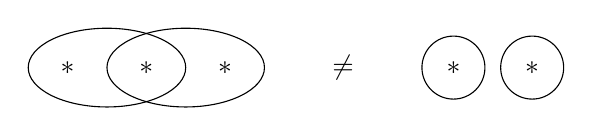
\begin{tikzpicture}
            \draw (-0.5,0) circle [x radius=1cm, y radius=0.5cm];
            \draw (0.5,0) circle [x radius=1cm, y radius=0.5cm];

            \node at (-1,0) {$\ast$};
            \node at (0,0) {$\ast$};
            \node at (1,0) {$\ast$};

            \node at (2.5,0) {$\neq$};

            \begin{scope}[xshift=4.4cm]
                \draw (-0.5,0) circle[radius=0.4cm];
                \draw (0.5,0) circle[radius=0.4cm];

                \node at (-0.5,0) {$\ast$};
                \node at (0.5,0) {$\ast$};
            \end{scope}
        \end{tikzpicture}
    \end{center}
\end{solution}

\begin{problem}
    Zeigen Sie: Für alle~$n \geq 1$ gilt
    \begin{equation}
        \sum_{k=1}^n k^2 = \frac{n (n+1) (2n+1)}{6}.\label{prob:eqn:sumsquare}
    \end{equation}
\end{problem}

\begin{solution}
    \begin{proof}
        Wir führen eine vollständige Fallunterscheidung über~$n$ durch. Dabei ist~$A(n)$ \cref{prob:eqn:sumsquare}.

        \begin{itemize}
            \item \emph{Induktionsanfang}: Für~$n = 1$ ist $1^2 = \frac{1}{6} (1 \cdot 2 \cdot 3)$ wahr und folglich ist auch $A(1)$ wahr.
            \item \emph{Induktionsschritt}: Wenn~$A(n)$ gilt, gilt auch
            \begin{align*}
                \sum_{k=1}^{n+1} k^2 &= (n+1)^2 + \sum_{k=1}^n k^2 \overset{A(n)}{=} (n+1)^2 + \frac{n(n+1)(2n+1)}{6} = \frac{n+1}{6} \bigl(6(n+1) + n(2n+1)\bigr) \\
                &= \frac{n+1}{6} \bigl((4n+6) + n(2n+3)\bigr) = \frac{(n+1) (n+2) (2n+3)}{6},
            \end{align*}
            also ist auch~$A(n+1)$ wahr.\qedhere
        \end{itemize}
    \end{proof}

    Alternativ können wir das auch nicht induktiv über Teleskopsummen zeigen.

    \begin{proof}
        In der Summe heben sich der Minuend~$k^3$ des Index~$i$ mit dem Subtrahenden $-(k-1)^3$ des Index~$i+1$ auf. Damit gilt
        \begin{gather*}
            n^3 = \sum_{k=1}^n \paren*{k^3 - (k-1)^3} = 3\sum_{k=1}^n k^2 - 3\sum_{k=1}^n k + \sum_{k=1}^n 1 = 3\sum_{k=1}^n k^2 - 3\frac{n (n+1)}{2} + n \\
            \iff \sum_{k=1}^n k^2 = \frac{n^3}{3} + \frac{n^2}{2} + \frac{n}{6} = \frac{n (n+1) (2n+1)}{6}. \qedhere
    \end{gather*}
    \end{proof}
\end{solution}

\section{Körper}

Auch \emph{Rechenbereich} genannt. Körper verallgemeinern und abstrahieren die uns gewohnten rationalen oder reellen Zahlen und deren Rechenoperationen. Dennoch sollten wir uns ab sofort von den uns bekannten Beispielen lösen, da die in der (linearen) Algebra betrachteten Objekte sehr abstrakt werden und nicht unbedingt analog zu unserem Vorwissen funktionieren.

\subsection{Körperaxiome}

\begin{definition}[Körper]
    Ein \emph{Körper} ist eine Menge~$K$ zusammen mit zwei Abbildungen
    \begin{equation*}
        +\colon K \times K \to K,\quad (a, b) \mapsto a+b \quad\qquad\text{und}\qquad\quad \cdot\colon K \times K \to K,\quad (a, b) \mapsto a\cdot b,
    \end{equation*}
    \emph{Addition} bzw.\ \emph{Multiplikation} genannt, sodass folgende Regeln (Axiome) gelten:
    \begin{enumerate}[leftmargin=*, widest=(M0)]
        \refitem[(A1)] $a+(b+c) = (a+b)+c$ für alle $a, b, c \in K$ (\emph{Assoziativität der Addition});\label{ax:field:aa}
        \refitem[(A2)] $a+b = b+a$ für alle $a, b \in K$ (\emph{Kommutativität der Addition});\label{ax:field:ac}
        \refitem[(A3)] Es existiert ein Element $0 = 0_K \in K$ mit $a+0 = a$ für alle~$a \in K$ (Existenz eines \emph{Nullelements});\label{ax:field:an}
        \refitem[(A4)] Zu jedem~$a \in K$ gibt es ein~$-a \in K$ mit $a+(-a) = 0$ (Existenz eines \emph{additiven Inversen});\label{ax:field:ai}
        \refitem[(M1)] $a\cdot(b\cdot c) = (a\cdot b)\cdot c$ für alle $a, b, c \in K$ (\emph{Assoziativität der Multiplikation});\label{ax:field:ma}
        \refitem[(M2)] $a\cdot b = b\cdot a$ für alle $a, b \in K$ (\emph{Kommutativität der Multiplikation});\label{ax:field:mc}
        \refitem[(M3)] Es existiert ein Element $1 = 1_K \in K$ mit~$1 \neq 0$ und $1\cdot a = a$ für alle~$a \in K$ (Existenz eines \emph{Einselements});\label{ax:field:mn}
        \refitem[(M4)] Zu jedem~$a \in K$ mit~$a \neq 0$ gibt es ein~$a^{-1} \in K$ mit~$a\cdot a^{-1} = 1$ (Existenz des \emph{multiplikativen Inversen});\label{ax:field:mi}
        \refitem[(D)] $(a+b)\cdot c = (a\cdot c)+(b\cdot c)$ für alle $a, b, c \in K$ (\emph{Distributivität}).\label{ax:field:d}
    \end{enumerate}
\end{definition}

Oftmals lassen wir den Index~$K$ wie in $0_K$~und~$1_K$ weg, wenn der Kontext klar ist. Manchmal schreiben wir ihn aber hinzu, um zu verdeutlichen, dass sie zum Körper~$K$ gehören.

\begin{remark}
    Wir setzen $1 \neq 0$ voraus, d.\,h.\ ein Körper hat mindestens zwei Elemente.\footnote{Traditionell wird in der Algebra $1 \neq 0$ definiert. Es gibt aber "`esoterische"' Konzepte eines einelementigen Körpers~$\F_1$, d.\,h.\ $1 = 0$, was aber einige Körpereigenschaften verliert.}
\end{remark}

\begin{remark}
    Dabei steht der Ausdruck~$a+b$ eigentlich für~$+\bigl((a, b)\bigr)$ und~$a\cdot b$ für~$\cdot\bigl((a, b)\bigr)$. Streng genommen müssten wir z.\,B.\ die Assoziativität der Addition~\ref{ax:field:aa} als
    \begin{equation*}
        a+(b+c) = (a+c)+b \quad\longrightarrow\quad  +\Bigl(\!\bigl(a, +\bigl((b, c)\bigr)\bigr)\!\Bigr) = +\Bigl(\!\bigl(+\bigl((a, b)\bigr), c\bigr)\!\Bigr)
    \end{equation*}
    und die Kommutativität der Addition~\ref{ax:field:ac} als
    \begin{equation*}
        a+b = b+a \quad\longrightarrow\quad +\bigl((a, b)\bigr) = +\bigl((b, a)\bigr)
    \end{equation*}
    schreiben.
\end{remark}

\begin{notation}\label{not:field:convention}
    Neben diesen Axiomen führen wir noch einige Konventionen ein.
    \begin{itemize}
        \item Um Klammern zu sparen, gilt \emph{Punktrechnung vor Strichrechnung}. Damit können wir z.\,B.\ das Distributivgesetz~\ref{ax:field:d} umschreiben als $a\cdot c + b\cdot c$, ohne dass Verwirrung entsteht.
        \item Wir definieren $a-b \coloneqq a+(-b)$ und $ab \coloneqq a\cdot b$ für $a, b \in K$. Somit können wir Plusklammern und Malpunkte weglassen, wenn der Sinn dabei nicht verfälscht wird (z.\,B.\ nicht $1 \cdot 2 \neq 12$).
        \item Für $a, b \in K$ mit~$b \neq 0$ sei
        \begin{equation*}
            \frac{a}{b} \coloneqq a/b \coloneqq a \cdot b^{-1}.
        \end{equation*}
    \end{itemize}
\end{notation}

Diese Regeln und Schreibweisen sind alles Konventionen und hängen nicht mit der Struktur oder den Eigenschaften eines Körper zusammen. Wir hätten genauso jede andere Konvention einführen können.

\begin{notation}
    Wir definieren kurz $K^\times \coloneqq K \setminus \mset{0}$.
\end{notation}

Ab sofort meinen wir mit~$K$ immer einen Körper mit den Operationen $+$~und~$\cdot$, falls nicht anders spezifiziert. Manchmal schreiben wir auch $(K, +, \cdot)$ für einen Körper.

\subsection{Beispiele von Körpern}

\begin{example}
    $\Q$~und~$\R$ mit den üblichen Abbildungen $+$~und~$\cdot$ sind Körper.
\end{example}

\begin{example}
    $\Z$~ist kein Körper, da (nur)~\ref{ax:field:mi} nicht erfüllt wird.
\end{example}

\begin{example}
    $\C$, die Menge der komplexen Zahlen mit $+$~und~$\cdot$ ist ein Körper.
\end{example}

\begin{example}
    Sei $K \coloneqq \mset{a, b}$ mit~$a \neq b$. Wir definieren die Abbildungen $+\colon K \times K \to K$ und $\cdot\colon K \times K \to K$ durch\footnote{Die Abbildungen ähneln der Addition und Multiplikation modulo~2.}
    \begin{align*}
        a + a &= a, & a + b &= b, & b + a &= b, & b + b &= a, \\
        a \cdot a &= a, & a \cdot b &= a, & b \cdot a &= a, & b \cdot b &= b.
    \end{align*}
    $K$~erfüllt alle Axiome eines Körpers, wobei das Nullelement~$0_K = a$ und das Einselement~$1_K = b$ ist, also $K = \F_2 \coloneqq \mset{0, 1}$. Der Körper ist der kleinstmögliche Körper (jeder Körper muss mindestens 0~und~1 enthalten). Tatsächlich ist der Körper sogar eindeutig, was wir aber nicht beweisen werden.
\end{example}

\begin{example}
    Sei~$K \coloneqq \Q(\sqrt{2}) \coloneqq \mset{a+b\sqrt{2} \mid a, b \in \Q} \subset \R$.\footnote{Das ist eine sog.\ Körperadjunktion bzw.\ Körpererweiterung} Wir definieren die Abbildungen $+\colon K \times K \to K$ und $\cdot\colon K \times K \to K$ als Einschränkung von $+\colon \R \times \R \to \R$ und $\cdot\colon \R \times \R \to \R$ (d.\,h.\ die Abbildungen sind dieselben aus~$\R$ bis auf den kleineren Definitionsbereich). Insbesondere heißt das
    \begin{gather*}
        (a+b\sqrt{2}) + (c+d\sqrt{2}) \coloneqq (a+c) + (b+d)\sqrt{2}
        \shortintertext{und}
        (a+b\sqrt{2}) \cdot (c+d\sqrt{2}) \coloneqq (ac+2bd) + (ad+bc)\sqrt{2}.
    \end{gather*}

    Die meisten Körperaxiome sind offensichtlich erfüllt. Für~\ref{ax:field:mi} stellt sich jedoch die Frage, ob $(a+b\sqrt{2})^{-1} \in K$ für alle~$a+b\sqrt{2} \neq 0$ existiert. \emph{Antwort}: Ja, denn
    \begin{gather*}
        (a+b\sqrt{2}){-1} \coloneqq \frac{a}{a^2-2b^2} + \frac{-b}{a^2-2b^2} \sqrt{2}
        \shortintertext{mit}
        \frac{a}{a^2-2b^2} + \frac{-b}{a^2-2b^2} \sqrt{2} = \frac{a-b\sqrt{2}}{a^2-2b^2} = \frac{a-b\sqrt{2}}{(a+b\sqrt{2}) (a-b\sqrt{2})} = \frac{1}{a+b\sqrt{2}}.
    \end{gather*}

    \emph{Beachte}: Die Brüche sind definiert, weil $(a/b)^2 \neq 2 \iff a^2-2b^2 \neq 0$ wegen~$\sqrt{2} \notin \Q$.
\end{example}

\subsection{Rechenregeln in Körpern}

\begin{lemma}[Linksdistributivität]
    Es gilt $a(b+c) = ac+ac$ für alle $a, b, c \in K$.
\end{lemma}

\begin{proof}
    Es gilt $a(b+c) \overset{\text{\ref{ax:field:mc}}}{=} (b+c)a \overset{\text{\ref{ax:field:d}}}{=} ba+ca \overset{\text{\ref{ax:field:mc}}}{=} ab+ac$.
\end{proof}

\begin{lemma}[Eindeutigkeit der Null]
    Es gibt nur ein Nullelement in einem Körper.
\end{lemma}

\begin{proof}
    Seien $0'$~und~$0''$ Nullelemente im Körper~$K$. Dann gilt $0'' \overset{\text{\ref{ax:field:an}}}{=} 0''+0' \overset{\text{\ref{ax:field:ac}}}{=} 0'+0'' \overset{\text{\ref{ax:field:an}}}{=} 0'$. Dabei haben wir für die erste Gleichheit die Eigenschaft $0' = 0_K$ und für die letzte Gleichheit $0'' = 0_K$ ausgenutzt.
\end{proof}

\begin{lemma}
    Für alle~$a \in K$ gilt $0a = 0$.
\end{lemma}

\begin{proof}
    Sei~$a \in K$. Dann gelten
    \begin{gather}
        0a \overset{\text{\ref{ax:field:an}}}{=} (0+0)a \overset{\text{\ref{ax:field:d}}}{=} 0a + 0a, \label{eqn:fieldprop:timeszero}\\
        0 \overset{\text{\ref{ax:field:ai}}}{=} 0a + (-(0a)) \overset{\text{\eqref{eqn:fieldprop:timeszero}}}{=} (0a + 0a) + (-(0a)) \overset{\text{\ref{ax:field:aa}}}{=} 0a + (0a + (-(0a))) \overset{\text{\ref{ax:field:ai}}}{=} 0a + 0 \overset{\text{\ref{ax:field:an}}}{=} 0a. \tag*{\qedhere}
    \end{gather}
\end{proof}

In den Übungsaufgaben werden wir noch eine Vielzahl weiterer Regeln beweisen.

\subsection{Charakteristik eines Körpers}

\begin{notation}
    Sei $K$~ein Körper. Für~$a \in K$ und $0 \neq m \in \N$ definieren wir
    \begin{equation*}
        m \cdot a \coloneqq \underbrace{a + a + \dots + a }_\text{$m$ mal}.
    \end{equation*}
\end{notation}

\begin{definition}[Charakteristik]
    Wir definieren $\mchar(K)$ als die \emph{Charakteristik} von~$K$ als
    \begin{equation*}
        \mchar(K) \coloneqq \begin{cases}
            0 & \text{falls $m \cdot 1_K \neq 0_K$ für alle $m \in \N \setminus \mset{0}$}, \\
            \min\mset{m \in \N \setminus \mset{0} \mid m \cdot 1_K = 0_K} & \text{sonst}.
        \end{cases}
    \end{equation*}
\end{definition}

\begin{lemma}\label{lem:primechar}
    Sei $K$~ein Körper mit $\mchar(K) = p > 0$. Dann ist $p$~eine Primzahl.
\end{lemma}

\begin{proof}
    Angenommen $p$~wäre keine Primzahl, sodass es $p_1, p_2 \in \N$ mit $p_1, p_2 \geq 2$ und $p = p_1p_2$ gibt. Aus der Minimalität der Charakteristik folgt $p_1 \cdot 1_K \neq 0$ und $p_2 \cdot 1_K \neq 0$. Damit gilt
    \begin{equation*}
        (p_1 \cdot 1_K) (p_2 \cdot 1_K) = (p_1p_2) \cdot 1_K = p \cdot 1_K = 0_K.
    \end{equation*}
    Aufgrund der Nullteilerfreiheit in einem Körper (s.~Übungsaufgabe) gilt $p_1 \cdot 1_K = 0_K$ oder $p_2 \cdot 1_K = 0_K$, ein Widerspruch.\footnote{Die Charakteristik hat einige interessante Eigenschaften:

    Aus einer positiven Charakteristik folgt sofort $a + a + \dots a = 0$. Sie hilft und zu bestimmen, wann ein Ausdruck Null wird, was wichtig für das Rechnen im Körper ist (wir denken an $a+0 = 0$, $0a = 0$ und, dass $0^{-1}$ nicht existiert). In diesem Kontext ist $\mchar(K) = 2$ besonders wichtig, denn in dem Fall ist $a + a = 0$ für alle~$a \in K$, d.\,h.\ jedes Element ist sein eigenes additives Inverse. $\mchar(K) \neq 2$ garantiert uns die Existenz der $2 \coloneqq 1+1$.
                
    Jeder Teilkörper eines Körpers hat dieselbe Charakteristik wie der Körper, z.\,B.\ $\mchar(\F_2) = \mchar(\F_4) = 2$. Damit haben Körper mit gleicher Charakteristik auch eine ähnliche Struktur.
                
    Die Charakteristik ist eigentlich für Ringe (die später folgen) definiert. All diese Eigenschaften gelten auch für Ringe.}
\end{proof}

\lecturesep{15.~Oktober 2021}

\subsection{Die Ringe~\texorpdfstring{$\bm{\Z_m}$}{Zm}}

\begin{definition}[Ring]
    Ein \emph{Ring} ist eine Menge~$R$ zusammen mit zwei Abbildungen
    \begin{equation*}
        +\colon R \times R \to R,\quad (a, b) \mapsto a+b \quad\qquad\text{und}\qquad\quad \cdot\colon R \times R \to R,\quad (a, b) \mapsto a \cdot b
    \end{equation*}
    \emph{Addition} bzw.\ \emph{Multiplikation} genannt, sodass folgende Regeln (Axiome) gelten:
    \begin{enumerate}[leftmargin=*, widest=(A1)]
        \refitem[(A1)] $a+(b+c) = (a+b)+c$ für alle $a, b, c \in R$ (\emph{Assoziativität der Addition});\label{ax:ring:aa}
        \refitem[(A2)] $a+b = b+a$ für alle $a, b \in R$ (\emph{Kommutativität der Addition});\label{ax:ring:ac}
        \refitem[(A3)] Es existiert ein Element $0 = 0_R \in R$ mit $a+0 = a$ für alle~$a \in R$ (Existenz eines \emph{Nullelements});\label{ax:ring:an}
        \refitem[(A4)] Zu jedem~$a \in R$ gibt es ein~$-a \in R$ mit $a+(-a) = 0$ (Existenz eines \emph{additiven Inversen});\label{ax:ring:ai}
        \refitem[(R1)] $a\cdot(b\cdot c) = (a\cdot b)\cdot c$ für alle $a, b, c \in R$ (\emph{Assoziativität der Multiplikation});\label{ax:ring:ma}
        \refitem[(R2)] Es existiert ein Element $1 = 1_R \in R$ mit~$1 \neq 0$ und $1\cdot a = a$ für alle~$a \in R$ (Existenz eines \emph{Einselements});\label{ax:ring:mn}
        \refitem[(D)] $(a+b)\cdot c = (a\cdot c)+(b\cdot c)$ und $a\cdot(b+c) = (a\cdot b)+(a\cdot c)$ für alle $a, b, c \in K$ (\emph{Distributivität}).\label{ax:ring:d}
    \end{enumerate}
\end{definition}

\begin{definition}[kommutativer Ring]
    Ein Ring~$R$ heißt \emph{kommutativ}, falls zusätzlich $a\cdot b = b\cdot a$ für alle $a, b \in \R$ gilt.
\end{definition}

\begin{remark}
    Im Vergleich zu einem Körper sind die Axiome der Addition identisch. Bei der Multiplikation fehlt lediglich die Kommutativität~\ref{ax:field:mc} und die Existenz des Inversen~\ref{ax:field:mi}. Aufgrund der fehlenden Kommutativität werden in der Distributivität beide Multiplikationsreihenfolgen angeben, die wir auch beide nachweisen müssen.
\end{remark}

\begin{remark}
    In einem Ring wird nicht verlangt, dass $1_R \neq 0_R$. Ist aber $1_R = 0_R$, so folgt daraus $a = 1_R a = 0_R a = 0_R$ für alle~$a \in R$, also $R = \mset{0_R}$.
\end{remark}

\begin{notation}[Nullring]
    Wir nennen $R = \mset{0_R}$ den trivialen\footnote{Als \emph{triviale} Objekte werden oft offensichtliche oder sehr einfache Objekte sowie uninteressante Randfälle bezeichnet.} \emph{Nullring}.
\end{notation}

Wir übernehmen für Ringe alle Schreibkonventionen in \cref{not:field:convention}, die wir für Körper festlegten (bis auf Brüche).

\begin{lemma}
    Seien $a, m \in \N$ mit~$m \geq 1$. Dann existieren eindeutig bestimmte Elemente $r, q \in \N$ mit $0 \leq r < m$, sodass $a = qm+r$ gilt. Setze $r_m(a) \coloneqq r$.
\end{lemma}

\begin{proof}
    Zu jedem~$a \in \N$ gibt es ein eindeutig bestimmtes~$q \in \N$ mit $qm \leq a < (q+1)m$. Mit $r \coloneqq a-qm$ folgt die Behauptung.
\end{proof}

\begin{definition}[$\Z$~modulo~$m$]
    Sei~$m \in \N$ mit~$m \geq 2$. Dann sei $\Z_m \coloneqq \mset{0, 1, \dots, m-1}$. Für $a, b \in \Z_m$ definieren wir noch Abbildungen $+$~und~$\cdot$ durch $a+b \coloneqq r_m(a\mathrel{+_{\,\Z}}b)$ und $a\cdot b \coloneqq r_m(a\mathrel{\cdot_{\,\Z}}b)$. (Die Operationen in den~$r_m(\dots)$ kommen aus~$\Z$.)
\end{definition}

Manchmal ist es hilfreich, auch die Operatoren aus verschiedenen Mengen durch Subskripte zu unterscheiden, also $+_K$, $\cdot_R$, etc.

\begin{lemma}
    $(\Z_m, +, \cdot)$ ist ein kommutativer Ring.\footnote{Ein sog.\ \emph{Restklassenring modulo~$m$}.}
\end{lemma}

\begin{proof}
    Übungsaufgabe.
\end{proof}

\begin{lemma}
    $(\Z_m, +, \cdot)$ ist genau dann ein Körper, wenn $m$~eine Primzahl ist.
\end{lemma}

\begin{proof}
    Angenommen $\Z_m$~ist ein Körper. Dann folgt $\mchar(\Z_m) = m$ aus der Definition der Addition über die Addition in~$\Z$ (in~$\Z$ ist $m1 = 1+1+\dots+1 = m$). Nach \cref{lem:primechar} ist $m$~eine Primzahl.

    Für die Umkehrung sei nun $m$~eine Primzahl. Zuerst zeigen wir, dass $\Z_m$ nullteilerfrei ist. Seien $a, b \in \Z_m$ mit $a\cdot b = 0 = r_m(a+b)$. Folglich wird $ab$ von~$m$ geteilt (Rest~0). Da $m$~eine Primzahl ist, folgt (aus dem \emph{Lemma von \textsc{Euklid}}): $m$~teilt~$a$ oder $m$~teilt~$b$. Weil nun $0 \leq a, b < m$ ist, muss $a = 0$ oder $b = 0$ sein. Folglich haben wir gezeigt, dass $\Z_m$~nullteilerfrei ist.

    Nun zeigen wir, dass jedes~$a \in \Z_m$ mit~$a \neq 0$ ein multiplikatives Inverses besitzt. Für solche~$a$ definieren wir die Abbildung $\rho_a\colon \Z_m \to \Z_m$, $x \mapsto xa$. Dann $\rho_a$~ist injektiv: Aus $xa = \rho_a(x) = \rho_a(y) = ya \iff (x-y)a = 0$ folgt aufgrund Nullteilerfreiheit $x-y = 0 \iff x = y$. Da $\Z_m$~endlich ist, ist $\rho_a$~auch surjektiv.

    Aus der Bijektion folgt, dass $0a, 1a, \dots, (m-1)a$ paarweise verschieden sind (injektiv), und diese Elemente auch jedes Element aus~$\Z_m$ repräsentiert (surjektiv), insbesondere die~1. Es gibt also ein~$x \in \Z_m$ mit~$xa = 1$. Zu jedem~$a \in \Z_m \setminus{0}$ gibt es also ein multiplikatives Inverses~$x \in \Z_m$, sprich $a$~ist invertierbar, was Axiom~\ref{ax:field:mi} erfüllt. Die restlichen Körperaxiome folgen aus dem kommutativen Ring.
\end{proof}

Vom kommutativen Ring zum Körper fehlt nur noch die Existenz des multiplikativen Inversen. Hierfür haben wir alle möglichen Kandidaten für das Inverse betrachtet, also $0a, 1a, \dots, (m-1)a$. Wir beobachten, dass diese Menge genau~$\Z_m$ entspricht, es also eine einfache Bijektion~$\rho_a$ geben muss, die wir auch beweisen haben. Der Trick hier war zu zeigen, dass $\Z_m$~nullteilerfrei ist (ein gutes Zeichen, da Nullteilerfreiheit eine Körpereigenschaft ist).

\begin{notation}[endlicher Körper]
    Für Primzahlen~$p$ schreiben wir auch $\F_p \coloneqq \Z_p$.
\end{notation}

\section{Vektorräume}

\emph{Vektorräume} sind wichtige Objekte, die in vielen Bereichen der Mathematik vorkommen. Das Ziel der linearen Algebra ist es, eine "`Theorie der Vektorräume"' zu entwickeln und dabei die Eigenschaften von Vektorräumen zu erforschen.

\subsection{Vektorraumaxiome}

\begin{definition}[Vektorraum]
    Sei $K$~ein Körper.  Ein \emph{Vektorraum über~$K$} oder \emph{$K$"~Vektorraum} ist eine Menge~$V$ zusammen mit zwei Abbildungen
    \begin{equation*}
        +\colon V \times V \to V,\quad (v_1, v_2) \mapsto v_1+v_2 \quad\qquad\text{und}\qquad\quad \cdot\colon K \times V \to V,\quad (a, v) \mapsto a\cdot v,
    \end{equation*}
    \emph{Addition} bzw.\ \emph{Skalarmultiplikation} genannt, sodass folgende Regeln (Axiome) gelten:
    \begin{enumerate}[leftmargin=*, widest=(SM0)]
        \refitem[(A1)] $v_1+(v_2+v_3) = (v_1+v_2)+v_3$ für alle $v_1, v_2, v_3 \in V$ (\emph{Assoziativität der Addition});\label{ax:vecspace:aa}
        \refitem[(A2)] $v_1+v_2 = v_2+v_1$ für alle $v_1, v_2 \in V$ (\emph{Kommutativität der Addition});\label{ax:vecspace:ac}
        \refitem[(A3)] Es existiert ein Element $0 = 0_V \in V$ mit $v + 0_V = v$ für alle~$v \in V$ (Existenz eines \emph{Nullelements});\label{ax:vecspace:an}
        \refitem[(A4)] Zu jedem~$v \in V$ gibt es ein~$-v \in V$ mit $v+(-v) = 0$ (Existenz eines \emph{additiven Inversen});\label{ax:vecspace:ai}
        \refitem[(SM1)] $(ab)\cdot v = a\cdot(b\cdot v)$ für alle $a, b \in K$ und~$v \in V$;\label{ax:vecspace:smcomp}
        \refitem[(SM2)] $1_K \cdot v = v$ für alle~$v \in V$;\label{ax:vecspace:smn}
        \refitem[(SM3)] $a\cdot(v_1+v_2) = a\cdot v_1 + a\cdot v_2$ für alle~$a \in K$ und $v_1, v_2 \in V$;\label{ax:vecspace:smdv}
        \refitem[(SM4)] $(a+b)\cdot v = (a\cdot v)+(b\cdot v)$ für alle~$a, b \in K$ und~$v \in V$.\label{ax:vecspace:smdf}
    \end{enumerate}
\end{definition}

Wir schreiben oft auch einfach~$V$ für den $K$"~Vektorraum $(V,+,\cdot)$.

\begin{notation}
    Um die Notation zu vereinfachen, legen wir $v_1-v_2 \coloneqq v_1+(-v_2)$, $av \coloneqq a \cdot v$ für alle $v_1, v_2, v \in V$ und $a \in K$ sowie \emph{Punkt"~ vor Strichrechnung} fest.
\end{notation}

\begin{notation}[Vektor, Skalar, Nullvektor]
    Die Elemente von~$V$ nennen wir \emph{Vektoren}, die Elemente von~$K$ nennen wir \emph{Skalare}. Das Nullelement~$0_V$ heißt \emph{Nullvektor} oder auch \emph{die Null von~$V$}.
\end{notation}

\begin{remark}
    Es ist sehr wichtig, zu wissen, welchen Grundkörper~$K$ der Vektorraum hat. Dieselbe Menge~$V$, aber über zwei verschiedene Körper $K_1$~und~$K_2$, sind zwei verschiedene Vektorräume, nämlich ein $K_1$"~ und ein $K_2$"~Vektorraum. Im Allgemeinen ist ein Vektorraum über einen anderen Körper kein Vektorraum mehr, da er z.\,B.\ nicht mehr abgeschlossen ist.
\end{remark}

\begin{remark}
    Die Skalarmultiplikation multipliziert ein Skalar mit einem Vektor (wie der Name schon sagt, also \underline{kein} Skalarprodukt). Wir beachten auch die Reihenfolge der Skalarmultiplikation, d.\,h.\ Skalare werden von \emph{links} multipliziert.
\end{remark}

Wie bei Körpern gibt es eine Vielzahl an Rechenregeln für Vektorräume, die wir in den Übungen beweisen.

\subsection{Beispiele von Vektorräumen}

\begin{notation}[Nullvektorraum]
    Sei $V \coloneqq \mset{0}$ über~$K$ der (triviale) \emph{Nullvektorraum} (oft auch einfach nur $V = 0$). Addition und Skalarmultiplikation können nur auf genau eine Weise definiert werden:
    \begin{gather*}
        +\colon V\times V \to V,\qquad 0+0 \mapsto 0 \\
        \cdot\colon V\times V \to V,\qquad 0\cdot0 \mapsto 0 \\
    \end{gather*}
\end{notation}

\begin{example}
    Sei $K$~ein Körper. Dann ist $K$ ein $K$"~Vektorraum mit Addition und Skalarmultiplikation definiert als Addition und Multiplikation von~$K$.
\end{example}

\begin{definition}[Standardvektorraum]
    Sei $K$~ein Körper. Für~$n \geq 1$ sei $V \coloneqq K^n$ das $n$"~fache kartesische Produkt von~$K$. Die Elemente aus~$K^n$ schreiben wir oft als Spalten
    \begin{equation*}
        \p{a_1\\\vdots\\a_n}
    \end{equation*}
    mit $a_1,\dots,a_n \in K$. Wir definieren komponentenweise
    \begin{gather*}
        +\colon V\times V \to V \quad\text{durch}\quad \paren*{\p{a_1\\\vdots\\a_n}, \p{b_1\\\vdots\\b_n}} \mapsto \p{a_1+b_1\\\vdots\\a_n+b_n}
        \shortintertext{und}
        \cdot\colon K\times V \to V \quad\text{durch}\quad \paren*{a, \p{b_1\\\vdots\\b_n}} \mapsto \p{ab_1\\\vdots\\ab_n}.
    \end{gather*}
    
    Dann ist $(V,+,\cdot)$ ein $K$"~Vektorraum, der sog.\ \emph{Standardvektorraum}. Wir legen $K^0 \coloneqq 0$ aus~$K$ fest.

    Dabei stammt die komponentenweise Addition und Multiplikation aus~$K$.
\end{definition}

In~$V = \R^2$ mit~$K = \R$ können wir Addition und Skalarmultiplikation visualisieren, indem wir Vektoren als Pfeile darstellen. Addition heißt dann Aneinanderreihen von Pfeilen; Skalarmultiplikation heißt dann Strecken\slash Stauchen oder Änderung der Richtung von Pfeilen. Das sollte aus der Schule bekannt sein.
\begin{center}
    \begin{tikzpicture}
        \draw[->] (-2.5,0) -- (5,0) node[below] {$\R$};
        \draw[->] (0,-1.5) -- (0,2.5) node[left] {$\R$};
        \draw[->] (0,0) -- (-2,1) node[left] {$v$};
        \draw[->] (0,0) -- (2,-1) node[below left] {$-v$};
        \draw[->] (0,0) -- (3,1) node[below right] {$w$};
        \draw[->] (0,0) -- (4.5,1.5) node[below right] {$\frac{3}{2}w$};
        \draw[->] (0,0) -- (1,2) node[above] {$v+w$};
        \draw[dashed] (-2,1) -- (1,2) -- (3,1);
    \end{tikzpicture}
\end{center}

Ein sehr wichtiges Beispiel von Vektorräumen:

\begin{definition}[Funktionenraum]
    Sei $K$~ein Körper und sei $I \neq \varnothing$ eine Menge. Wir setzen $V \coloneqq K^I \coloneqq \map(I, K)$ und definieren
    \begin{gather*}
        +\colon V \times V \to V,\quad (f,g) \mapsto f+g \quad\qquad\text{und}\qquad\quad \cdot\colon K \times V \to V,\quad (a,f) \mapsto af,
        \shortintertext{punktweise durch}
        (f+g)(x) \coloneqq f(x)+g(x) \quad\qquad\text{und}\qquad\quad (af)(x) \coloneqq a(f(x))
    \end{gather*}
    für alle $f,g \in V$, $a \in K$, und $x \in I$.

    Dann ist $(V,+,\cdot)$ ein $K$"~Vektorraum, der sog.\ \emph{(lineare) Funktionenraum}. Wir definieren $K^\varnothing = 0$ als Nullabbildung.
\end{definition}

Dabei ist in den Definitionsgleichungen auf der linken Seite Addition und Skalarmultiplikation in~$V$, sowie auf der rechten Seite Addition und Multiplikation in~$K$.\footnote{An dieser Stelle fragt man sich vielleicht, warum der Standardvektorraum~$K^n$ und der Funktionenraum~$K^I$ identisch notiert werden. Das liegt daran, dass sie tatsächlich "`identisch"' (d.\,h.\ \emph{isomorph}) sind, weil es eine Bijektion wie in \cref{ex:map:setisoproduct} gibt.}\textsuperscript{,}\footnote{Für~$I = \N$ lässt sich auch der "`unendlichdimensionale"' \emph{Folgenraum}
\begin{equation*}
    K^\N \coloneqq \mset{(a_1,a_2,a_3,\dots) \mid a_i \in K \text{ für alle } i \in \N}
\end{equation*}
(wie in der Analysis) definieren.}

Ein noch wichtigeres Beispiel ist

\begin{definition}
    Sei $K$~ein Körper und sei $I \neq \varnothing$ eine Menge. Dann ist
    \begin{equation*}
        K^{(I)} \coloneqq \mset{f \in K^I \mid f(x) \neq 0 \text{ für nur endlich viele } x \in I}
    \end{equation*}
    ein $K$"~Vektorraum, wobei wir Addition und Skalarmultiplikation von~$K^I$ benutzen. Wir definieren $K^{(\varnothing)} = 0$ als Nullabbildung.
\end{definition}

Jede Abbildung $f \in K^{(I)}$ bildet also fast alle~$x \in I$ (bis auf endlich viele) auf~0 ab.

\begin{definition}[Teilkörper]
    Sei $(L,+,\cdot)$ ein Körper und sei $K$~eine Teilmenge von~$L$, sodass die Eigenschaften
    \begin{enumerate}
        \item $0, 1 \in K$ (neutrale Elemente);
        \item $a+b \in K$ für alle $a,b \in K$ (Abgeschlossenheit unter Addition);\label{def:subfield:add}
        \item $a\cdot b \in K$ für alle $a,b \in K$ (Abgeschlossenheit unter Multiplikation);\label{def:subfield:mul}
        \item $-a \in K$ für alle~$a \in K$ (additive Inverse) und
        \item $a^{-1} \in K$ für alle~$a \in K^\times$ (multiplikative Inverse)
    \end{enumerate}
    erfüllt sind. Durch Einschränkung erhalten wir die Abbildungen
    \begin{equation*}
        +\colon K\times K \to K \quad\qquad\text{und}\qquad\quad \cdot\colon K\times K \to K.
    \end{equation*}
    (Das ist aufgrund der Abgeschlossenheit von $+$~und~$\cdot$ garantiert, s.~\cref{def:subfield:add,def:subfield:mul}.) Wir können leicht überprüfen, dass $K$~einen Körper bildet, und nennen~$K$ einen \emph{Teilkörper} von~$L$.
\end{definition}

\begin{example}
    Ist $K$~ein Teilkörper von~$L$, so ist $L$~ein $K$"~Vektorraum, wobei die Skalarmultiplikation $\cdot\colon K\times L \to L$ durch Einschränkung der Multiplikation $\dot\colon L\times L \to L$ definiert ist.

    Bspw.\ ist der Körper~$\Q(\sqrt{2})$ ein $\Q$"~Vektorraum und $\R$~sowohl ein~$\Q$"~ als auch ein $\Q(\sqrt{2})$"~Vektorraum.
\end{example}

\begin{definition}[externe direkte Summe]
    Seien $V$~und~$W$ zwei $K$"~Vektorräume. Dann ist die $V \times W$ wieder ein $K$"~Vektorraum, wobei Addition und Skalarmultiplikation komponentenweise definiert sind durch
    \begin{gather*}
        (v_1,w_1) + (v_2,w_2) \coloneqq (v_1+v_2, w_1+w_2) \qquad\text{und}\qquad a(v,w) \coloneqq (av, aw)
    \end{gather*}
    für alle $v,v_1,v_2 \in V$, $w,w_1,w_2 \in W$ und $a \in K$. Der $K$"~Vektorraum $V \times W$ nennen wir die \emph{(externe) direkte Summe} von $V$~und~$W$ und schreiben $V \oplus W$.
\end{definition}

Noch ein Beispiel aus der Analysis.

\begin{example}
    Sei $I = [a,b]$ ein abgeschlossenes Intervall in~$\R$ und sei
    \begin{equation*}
        C^0(I) \coloneqq \mset{\text{stetige Funktionen } I \to \R}
    \end{equation*}
    eine Teilmenge von~$\R^I$. Dann ist $C^0(I)$~ein $\R$"~Vektorraum mit der Einschränkung von $+\colon \R^I\times\R^I \to \R^I$ und $\cdot\colon \R\times\R^I \to \R^I$ auf die neue Definitionsmenge~$I \subset \R$.
\end{example}

\lecturesep{19.~Oktober 2021}

\subsection{Unterräume}

\begin{definition}
    Sei $V$~ein $K$"~Vektorraum. Eine Teilmenge~$U$ von~$V$ heißt \emph{Unterraum} von~$V$, falls gilt:
    \begin{enumerate}
        \item $U \neq \varnothing$;
        \item $u_1+u_2 \in U$ für alle $u_1,u_2 \in U$ und\label{def:subspace:add}
        \item $au \in U$ für alle~$a \in K$ und~$u \in U$.\label{def:subspace:mul}
    \end{enumerate}
\end{definition}

\begin{lemma}
    Sei $U$~ein Unterraum von~$V$. Durch Einschränkung der Addition und Skalarmultiplikation von~$V$ erhalten wir Abbildungen $+\colon U\times U \to U$ und $\cdot\colon K\times U \to U$ (was aufgrund \cref{def:subfield:add,def:subfield:mul} möglich ist). Dann ist $U$ zusammen mit beiden Einschränkungen wieder ein $K$"~Vektorraum.
\end{lemma}

\begin{proof}
    Sei~$u \in U$. Aus \cref{def:subfield:mul} folgen $0u = 0 \in U$ und $(-1)u = -u \in U$. Deshalb gelten die Vektorraumaxiome \ref{ax:vecspace:an}~und~\ref{ax:vecspace:ai}. Alle anderen Axiome folgen aus~$V$.
\end{proof}

\begin{example}
    Die Teilmengen~$V$ und~$\mset{0}$ (statt~$\mset{0}$ schreiben wir oft nur~0) sind Unterräume von~$V$, die sog.\ \emph{trivialen Unterräume}.
\end{example}

\begin{example}
    Sei~$v \in V$. Dann ist
    \begin{equation*}
        U_v \coloneqq Kv \coloneqq \mset{av \mid a \in K}
    \end{equation*}
    der kleinste Unterraum\footnote{An der Stelle müssten wir definieren, was "`klein"' i.\,S.\,v.\ Unterräumen bedeuten soll. Hier meint der Dozent wahrscheinlich die \emph{Dimension}, die später drankommt.} von~$V$, welcher $v$~enthält.
\end{example}

\begin{definition}[Gerade]
    Ist~$v \neq 0$, so nennen wir
    \begin{equation*}
        U_v \coloneqq Kv \coloneqq \mset{av \mid a \in K}
    \end{equation*}
    die durch~$v$ verlaufende \emph{Gerade}.
\end{definition}

\begin{example}
    Für jede Menge~$I$ ist $K^{(I)}$~ein Unterraum von~$K^I$, denn nach Addition und Skalarmultiplikation hat jede Abbildung immer noch nur endlich viele Stellen ungleich~0.
\end{example}

\begin{example}
    Sei $I = [a,b]$ ein Intervall in~$\R$. Dann ist $C^0(I)$~ein Unterraum von~$\R^I$, weil sich die Stetigkeit unter Addition und Skalarmultiplikation nicht ändert.
\end{example}

\begin{example}
    Die Elemente des $\R$"~Vektorraums~$\R^\N$ sind die in der Analysis behandelten reellen Folgen. Die Teilmenge der konvergenten reellen Folgen ist ein Unterraum von~$\R^\N$, da aufgrund der Grenzwertsätze die Folgen nach Addition und Skalarmultiplikation immer noch konvergieren.
\end{example}

\begin{example}
    Sei~$a \in K$. Wir definieren
    \begin{equation*}
        U(a) \coloneqq \mset*{\p{a\\b} \mid b \in K}.
    \end{equation*}
    Dann ist $U(a)$ genau dann ein Unterraum von~$K^2$, wenn $a = 0$.
\end{example}

\begin{definition}[Durchschnitt, Summe]
    Seien $U_1$~und~$U_2$ Unterräume von~$V$. Dann ist $U_1 \cap U_2$ der \emph{Durchschnitt} von $U_1$~und~$U_2$ sowie
    \begin{equation*}
        U_1+U_2 \coloneqq \mset{u_1+u_2 \mid u_1 \in U_1, u_2 \in U_2}
    \end{equation*}
    die \emph{Summe} von $U_1$~und~$U_2$.
\end{definition}

\begin{lemma}
    $U_1 \cap U_2$ und $U_1+U_2$ sind Unterräume von~$V$.
\end{lemma}

\begin{definition}[interne direkte Summe]
    Seien $U_1$~und~$U_2$ Unterräume von~$V$. Ist $U_1 \cap U_2 = 0$, so nennen wir
    \begin{equation*}
        U_1\oplus U_2 \coloneqq U_1+U_2
    \end{equation*}
    die \emph{(interne) direkte Summe} von $U_1$~und~$U_2$.
\end{definition}

\begin{definition}[Summe, interne direkte Summe von Familien]
    Sei $I$~eine Indexmenge, und für jedes~$i \in I$ sei $U_i$~ein Unterraum von~$V$ (kurz $(U_i)_{i\in I}$ eine Familie von Unterräumen von~$V$). Die \emph{Summe}
    \begin{equation*}
        \sum_{i\in I} U_i
    \end{equation*}
    der Unterräume~$U_i$ ist die Menge aller Vektoren~$v \in V$, für die es eine endliche Teilmenge~$J \subseteq I$ gibt, sodass
    \begin{equation*}
        v = \sum_{j\in J} u_j \qquad\text{mit } u_j \in U_j \text{ für alle } j \in J.
    \end{equation*}

    Ist
    \begin{equation*}
        U_j \cap \paren*{\sum_{i\in I\setminus{j}} U_i} = 0 \qquad\text{für alle } j \in I,
    \end{equation*}
    so nennen wir die Summe \emph{(interne) direkte Summe} und schreiben
    \begin{equation*}
        \bigoplus_{i\in I} U_i \coloneqq \sum_{i\in I} U_i.
    \end{equation*}
\end{definition}

Jedes $v \in (U_i)_{i\in I}$ ist also eine Summe von endlich vielen Vektoren~$u_j$, wobei jedes~$u_j$ von einem anderen Unterraum kommt.\footnote{Anders formuliert: Jeder Vektor~$v$ der internen Summe ist die Summe $\sum_{i\in I} u_i$ mit $u_i \in U_i$, wobei $u_i \neq 0$ nur für endlich viele~$u_i$ gilt. Vgl.\ mit der Definition von~$K^{(I)}$.}\textsuperscript{,}\footnote{Eine witzige Eigenschaft: Für zwei Untervektorräume $U$~und~$W$ von~$V$ gilt
\begin{equation*}
    U\times\mset{0} \oplus \mset{0}\times W = U \oplus W,
\end{equation*}
also $(u, 0) + (0,w) = (u,w)$, wobei auf der linken Seite die \emph{interne} direkte Summe und auf der rechten Seite die \emph{externe} direkte Summe gemeint ist. Die Vektorräume auf der linken Seite teilen sich nur den Vektor $(0, 0)$.}

\begin{lemma}
    $\bigcup_{i\in I} U_i$ und $\sum_{i\in I} U_i$ sind Unterräume von~$V$.
\end{lemma}

Betrachten wir Standardvektorräume (wie z.\,B.~$\R^2$), dann können wir uns Untervektorräume als z.\,B.\ den Ursprung, Geraden, Ebenen, Räume, etc.\ vorstellen, die den Ursprung enthalten. Insbesondere sind $U_v$~Ursprungsgeraden. Die interne Summe zweier verschiedener Geraden in~$\R^2$ ist~$\R^2$ selbst; die Summe ist auch direkt, da sie nur~0 teilen.

\section{Lineare Abbildungen}

Die "`Theorie der Vektorräume"' wird interessant, wenn wir noch Abbildungen zwischen Vektorräumen betrachten. Dabei sollen sie die Vektorraumstruktur\footnote{Wichtig ist, dass die hier betrachteten Homomorphismen \emph{Vektorraumstrukturen} erhalten. Es gibt noch viele andere Homomorphismen, wie z.\,B.\ Mengenhomomorphismen (das sind die Abbildungen), Gruppenhomomorphismen, Homomorphismen zwischen topologischen Räumen (sog.\ Homöomorphismen), etc.} erhalten, d.\,h.\ mit der Addition und Skalarmultiplikation innerhalb des Start"~ und Zielvektorraums kompatibel sein. Das führt zu \emph{linearen Abbildungen} bzw.\ \emph{Homomorphismen} ("`Gleich-Gestalter"'). Das vorläufige Ziel wird es sein, lineare Abbildungen zu verstehen.

\subsection{Definition}

\begin{definition}[lineare Abbildung]
    Seien $V$~und~$W$ zwei $K$"~Vektorräume. Eine Abbildung $f\colon V \to W$ heißt \emph{linear} (oder \emph{$K$"~linear}), falls folgende Bedingungen gelten:
    \begin{enumerate}
        \item $f(v_1+v_2) = f(v_1)+f(v_2)$ für alle $v_1,v_2 \in V$; und
        \item $f(av) = af(v)$ für alle~$v \in V$ und~$a \in K$.
    \end{enumerate}
\end{definition}

Dabei finden Addition und Skalarmultiplikation zwischen den Argumenten der Abbildung in~$V$ und zwischen den Bildern der Abbildung in~$W$ statt. Anders geschrieben:
\begin{align*}
    f(v_1\mathrel{+_V}v_2) &= f(v_1)\mathrel{+_W}f(v_2), \\
    f(a\mathrel{\cdot_V}v) &= a\mathrel{\cdot_W}f(v)
\end{align*}

\begin{definition}[Homomorphismus, Endomorphismus]
    Ist~$f\colon V \to W$ linear, so nennen wir~$f$ einen \emph{Homomorphismus}. Ist zudem $V = W$, so nennen wir~$f$ einen \emph{Endomorphismus} (also $f\colon V \to V$).

    Weiterhin definieren wir
    \begin{gather*}
        \hom(V,W) \coloneqq \mset{f \in \map(V,W) \mid f \text{ ist ein Homomorphismus}}
        \shortintertext{und}
        \mend(V) \coloneqq \hom(V,V).
    \end{gather*}
\end{definition}

\begin{definition}[Monomorphismus, Epimorphismus, Isomorphismus]
    Sei $f\colon V \to W$ ein Homomorphismus.
    \begin{itemize}
        \item $f$~ist ein \emph{Monomorphismus}, falls $f$~injektiv ist.
        \item $f$~ist ein \emph{Epimorphismus}, falls $f$~surjektiv ist.
        \item $f$~ist ein \emph{Isomorphismus}, falls $f$~bijektiv ist.
    \end{itemize}
\end{definition}

\begin{definition}[isomorph]
    Zwei $K$~Vektorräume $V$~und~$W$ heißen \emph{isomorph}, falls ein Isomorphismus $f\colon V \to W$ existiert. Wir schreiben dann $V \cong W$.
\end{definition}

Der Begriff der Isomorphie ist sehr mächtig, da er uns erlaubt, innerhalb der linearen Algebra die beiden Objekte "`gleichzusetzen"', d.\,h.\ die Objekte sind zueinander äquivalent und verhalten sich auch (unter Addition und Skalarmultiplikation) gleich.

\begin{lemma}\label{lem:hom:def}
    Seien $V$~und~$W$ zwei $K$"~Vektorräume. Eine Abbildung $f\colon V \to w$ ist genau dann linear, wenn
    \begin{equation*}
        f(a_1v_1 + a_2v_2) = a_1f(v_1) + a_2f(v_2)
    \end{equation*}
    für alle $a_1,a_2 \in K$ und $v_1,v_2 \in V$ gilt.
\end{lemma}

\begin{proof}
    Übungsaufgabe.
\end{proof}

\subsection{Beispiele von linearen Abbildungen}

\begin{definition}[Nullabbildung]
    Seien $V$~und~$W$ zwei $K$"~Vektorräume. Die \emph{Nullabbildung}
    \begin{equation*}
        f\colon V \to W,\quad v \mapsto 0 \quad\text{für alle } v \in V
    \end{equation*}
    ist ein Homomorphismus. Wir schreiben $f = 0$.
\end{definition}

\begin{definition}[Identität]
    Sei $V$~ein $K$"~Vektorraum. Die \emph{Identität}
    \begin{equation*}
        f\colon V \to V,\quad v \mapsto v \quad\text{ für alle } v \in V
    \end{equation*}
    ist ein Homomorphismus. Wir schreiben $f = \id_V$.
\end{definition}

Die Identität ist ein bijektiver Endomorphismus, also ein Isomorphismus und insbesondere ein Homomorphismus.

\begin{example}\leavevmode
    \begin{enumerate}
        \item Sei $V$~ein $K$"~Vektorraum und sei~$a \in K$. Die Abbildung $f_a\colon V \to V$, $v \mapsto av$ für alle~$v \in V$ ist ein Homomorphismus. Ist $a \neq 0$, d.\,h.\ $f_a \neq 0$, so ist $f_a$~sogar ein Isomorphismus.
        \item Für jeden Homomorphismus $f\colon K \to K$ gibt es ein~$a \in K$ mit~$f = f_a$. Für alle~$\lambda \in K$ gilt nämlich $f(\lambda) = f(\lambda1) = \lambda f(1)$. Dann können wir $a \coloneqq f(1)$ setzen.
        \item Die Graphen der Homomorphismen $f\colon K \to K$ sind genau die Geraden~$U_v \subseteq K^2$, wobei $v = (a,b)$ mit~$a \neq 0$ ist. Die Punkte des Graphen sind nämlich $(\lambda,f(\lambda)) = (\lambda,\lambda f(1)) = \lambda(1,f(1))$ für alle~$\lambda \in K$. Für~$a = 0$ wäre $f$~nur auf~$0$ definiert.
    \end{enumerate}
\end{example}

\begin{example}
    Sei $K$~ein Körper und sei $(a,b,c,d) \in K^4$ gegeben. Die Abbildung
    \begin{equation*}
        f\colon K^2 \to K^2,\quad \p{x\\y} \mapsto \p{ax+by\\cx+dy}
    \end{equation*}
    ist ein Homomorphismus.

    (Um das nachzuweisen, setzen wir einfach in die Definition linearer Abbildungen ein. Für die Addition gilt
    \begin{equation*}
        f\paren*{\p{x_1\\y_1} + \p{x_2\\y_2}} = \p{a(x_1+x_2) + b(y_1+y_2) \\ c(x_1+x_2) + d(y_1+y_2)} = \p{ax_1+by_1\\cx_1+dy_1} + \p{ax_2+by_2\\cx_2+dy_2} = f\paren*{\p{x_1\\y_1}} + f\paren*{\p{x_2\\y_2}}.
    \end{equation*}
    Analog können wir zeigen, dass die Abbildung mit der Skalarmultiplikation kompatibel ist.)
\end{example}

\begin{example}
    Die Abbildung $f\colon \R \to \R$, $x \mapsto x^2$ ist kein Homomorphismus bzw.\ nicht $\R$"~linear, denn z.\,B.\ gilt $16 = f(2+2) \neq f(2)+f(2) = 8$.
\end{example}

\emph{Warnung}: In der linearen Algebra gibt es viele verschiedene Nullen. Z.\,B.\ seien $V$~und~$W$ zwei $K$"~Vektorräume. $0$~kann nun die Null~$0_K$ in~$K$, die Null~$0_V$ in~$V$, die Null~$0_W$ in~$W$, die Nullabbildung $0\colon V \to W$ oder der triviale Unterraum~$\mset{0}$ sein.

\subsection{Erste Eigenschaften linearer Abbildungen}

\begin{lemma}
    Sei $f\colon V \to W$ ein Homomorphismus. Dann gilt $f(0) = 0$.
\end{lemma}

\begin{proof}
    Es gibt zwei Möglichkeiten, die Aussage zu beweisen.

    Erster Beweis: Es gilt
    \begin{equation*}
        f(0) \overset{\ref{ax:vecspace:an}}{=} f(0+0) \overset{\text{Hom.}}{=} f(0)+f(0).
    \end{equation*}
    Daraus folgt
    \begin{equation*}
        0 \overset{\ref{ax:vecspace:ai}}{=} f(0)-f(0) = (f(0)+f(0)) - f(0) \overset{\ref{ax:vecspace:aa}}{=} f(0) + (f(0)-f(0)) \overset{\ref{ax:vecspace:ai}}{=} f(0)+0 \overset{\ref{ax:vecspace:an}}{=} f(0).
    \end{equation*}

    Zweiter Beweis: Für die Nullen $0_K \in K$, $0_V \in V$ und~$0_W \in W$ gilt mit der Rechenregel $0v = 0$
    \begin{equation*}
        f(0_V) = f(0_K0_V) \overset{\text{Hom.}}{=} 0_Kf(0_V) = 0_W. \qedhere
    \end{equation*}
\end{proof}

Der zweite Beweis ist zwar kürzer, ist aber weniger elementar.

\begin{lemma}
    Sei $f\colon V \to W$ ein Isomorphismus. Dann ist die Umkehrabbildung $f^{-1}\colon W \to V$ wieder ein Isomorphismus.
\end{lemma}

\begin{proof}
    Aus den Eigenschaften von Bijektionen wissen wir, dass~$f^{-1}$ existiert und auch bijektiv ist. Wir müssen noch zeigen, dass $f^{-1}$~linear ist.

    Weil $f$~bijektiv ist, ist jedes~$w \in W$ von der Form~$f(v) = w$ für ein eindeutig bestimmtes~$v \in V$. Dann gelten für alle $v,v_1,v_2 \in V$ und~$a \in K$
    \begin{gather*}
        f^{-1}(f(v_1) + f(v_2)) = f^{-1}(f(v_1+v_2)) = v_1+v_2 = f^{-1}(f(v_1)) + f^{-1}(f(v_2))
        \shortintertext{und}
        f^{-1}(a(f(v))) = f^{-1}(f(av)) = av = af^{-1}(f(v)).
    \end{gather*}
    Folglich ist $f^{-1}$~linear.
\end{proof}

\begin{lemma}
    Seien $f\colon U \to V$ und $g\colon V \to W$ Homomorphismen. Dann ist die Komposition $g\circ f\colon U \to W$ auch ein Homomorphismus.
\end{lemma}

\begin{proof}
    Wir verwenden \cref{lem:hom:def}. Für alle $a_1,a_2 \in K$ und $v_1,v_2 \in V$ gilt
    \begin{align*}
        (g\circ f)(a_1u_2 + a_2u_2) &= g(f(a_1u_1 + a_2u_2)) \overset{\text{Hom.~$f$}}{=} g(a_1f(u_1) + a_2f(u_2)) \\
        \overset{\text{Hom.~$g$}}&{=} a_1g(f(u_1)) + a_2g(f(u_2)) = a_1(g\circ f)(u_1) + a_2(g\circ f)(u_2). \qedhere
    \end{align*}
\end{proof}

\lecturesep{22.~Oktober 2021}

%\printsolutions

\newpage\appendix

\section{Trickkiste}



\end{document}
